%!TEX root = ../synopsis.tex

В {\bf первой главе}
проводится анализ проблемы автоматизированного проектирования УП
в раскройно-заготовительном производстве для оборудования термической фигурной резки с ЧПУ.
Описаны основные технологические особенности и ограничения термической резки,
которые необходимо соблюдать при проектировании УП.

\begin{figure}[h]
  \centering
  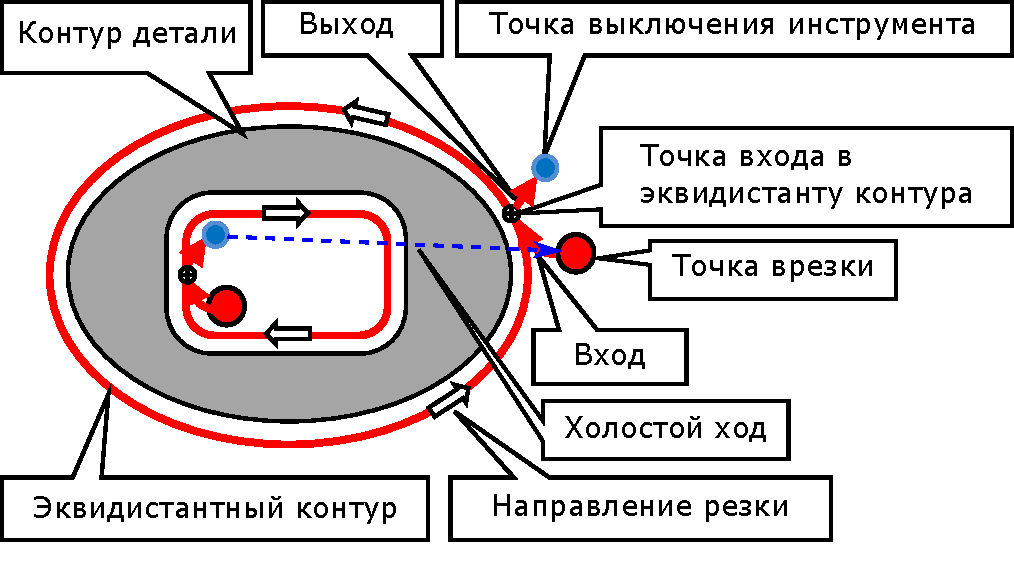
\includegraphics[width=0.8\textwidth]{toolpath.pdf}
  \caption{Элементы маршрута резки}
  \label{fig:toolpath}
\end{figure}

В общем случае маршрут инструмента содержит несколько компонент:
начальную $M_0$
и возможно отличную от неё конечную точку маршрута $M_{N+1}$,
$N$~точек врезки $M_i$, $i \in \overline{1, N}$
и соответствующих им точек выключения инструмента
$M_i^*$,
рабочий ход инструмента от точки врезки $M_i$
до точки выключения $M_i^*$
(в дальнейшем будем называть его траекторию
{\it сегментом резки}
$S_i=M_i M_i^*$)
а также холостой ход от $M_i^*$
до следующей точки врезки $M_{i+1}$,
см. рис.~\ref{fig:toolpath}.
В определение маршрута также входит
порядок резки,
то есть последовательность посещения точек врезки,
представляющая собой перестановку
$I = (i_1, i_2, ... i_N)$.
Таким образом,
маршрут резки можно определить
в терминах сегментов резки как кортеж
\begin{equation}
  \mathfrak{R} = \left<
    M_0, M_1, S_1, M_1^*, M_2, S_2, M_2^*, \,\dots, M_N, S_N, M_N^*,
    i_1, i_2, \,\dots, i_N
  \right>
  \label{eq:route:tuple}
\end{equation}

В качестве целевой функции при оптимизации часто используется время резки
\begin{equation}
  T_{cut} = \frac{L_{on}}{V_{on}} + \frac{L_{off}}{V_{off}} +N_{pt} \cdot t_{pt}
  ,
  \label{eq:cutting-time}
\end{equation}
где
$L_{on}$ -- длина реза с включенным режущим инструментом;
$V_{on}$ -- скорость рабочего хода режущего инструмента;
$L_{off}$ -- длина переходов с выключенным режущим инструментом (холостой ход);
$V_{off}$ -- скорость холостого хода;
$N_{pt}$ -- количество точек врезки;
$t_{pt}$ -- время, затрачиваемое на одну врезку.
В подавляющем большинстве исследований,
включая данную диссертационную работу,
$V_{on}$ считается константой
(в рамках конкретной УП),
однако вообще говоря это не так,
см.~\cite{Obuhovo}.

Важнейшей экономической характеристикой качества
разработанной управляющей программы является стоимость
(себестоимость) резки деталей на машине с ЧПУ.
По аналогии с \eqref{eq:cutting-time}
его можно определить по формуле:
\begin{equation}
  F_{cost}=
  L_{on} \cdot C_{on} +
  L_{off} \cdot C_{off} +
  N_{pt} \cdot C_{pt}
  ,
  \label{eq:cutting-cost}
\end{equation}
где
$C_{on}$ -- стоимость единицы пути с включенным режущим инструментом;
$C_{off}$ -- стоимость единицы пути с выключенным режущим инструментом;
$C_{pt}$ -- стоимость одной врезки.

Задача оптимизации маршрута инструмента для машин фигурной листовой резки с~ЧПУ
может быть представлена в общем виде
как задача минимизации некоторой числовой функции
$\mathfrak F$
(например, \eqref{eq:cutting-time} или \eqref{eq:cutting-cost})
на множестве
$\mathfrak G$ допустимых кортежей
\eqref{eq:route:tuple}:
\begin{equation}
  \mathfrak F(\mathfrak R) \to \min_{\mathfrak R \in \mathfrak G}
  \label{eq:cut:problem}
\end{equation}

В маршрут \eqref{eq:route:tuple} помимо перестановки
$I = (i_1, i_2, ... i_N)$.
входят также точки $M_i$ и $M_i^*$,
которые в общем случае должны ещё быть выбраны
из некоторого непрерывного множества,
что делает простую формулировку задачи \eqref{eq:cut:problem}
чрезвычайно сложной в решении.
Более того,
набор сегментов резки $S_i$
в общем случае не совпадает
(даже в количестве)
с набором контуров деталей,
подлежащих резке,
так как на практике используются различные техники резки:
\begin{enumerate}
  \item
  {\it Резка по замкнутому контуру (стандартная техника)}:
  в этом случае сегмент резки содержит
  ровно один замкнутый контур заготовки,
  который вырезается целиком.
  \item
  {\it Мультисегментная резка контура}:
  в этом случае для вырезки одного контура
  используются не менее двух сегментов резки.
  \item
  {\it Мультиконтурная резка}:
  резка предполагает вырезку нескольких
  контуров в одном сегменте.
\end{enumerate}

На рис.~\ref{fig:cut-classes}
представлена классификация задач резки\dots


\begin{figure}
  \centering
  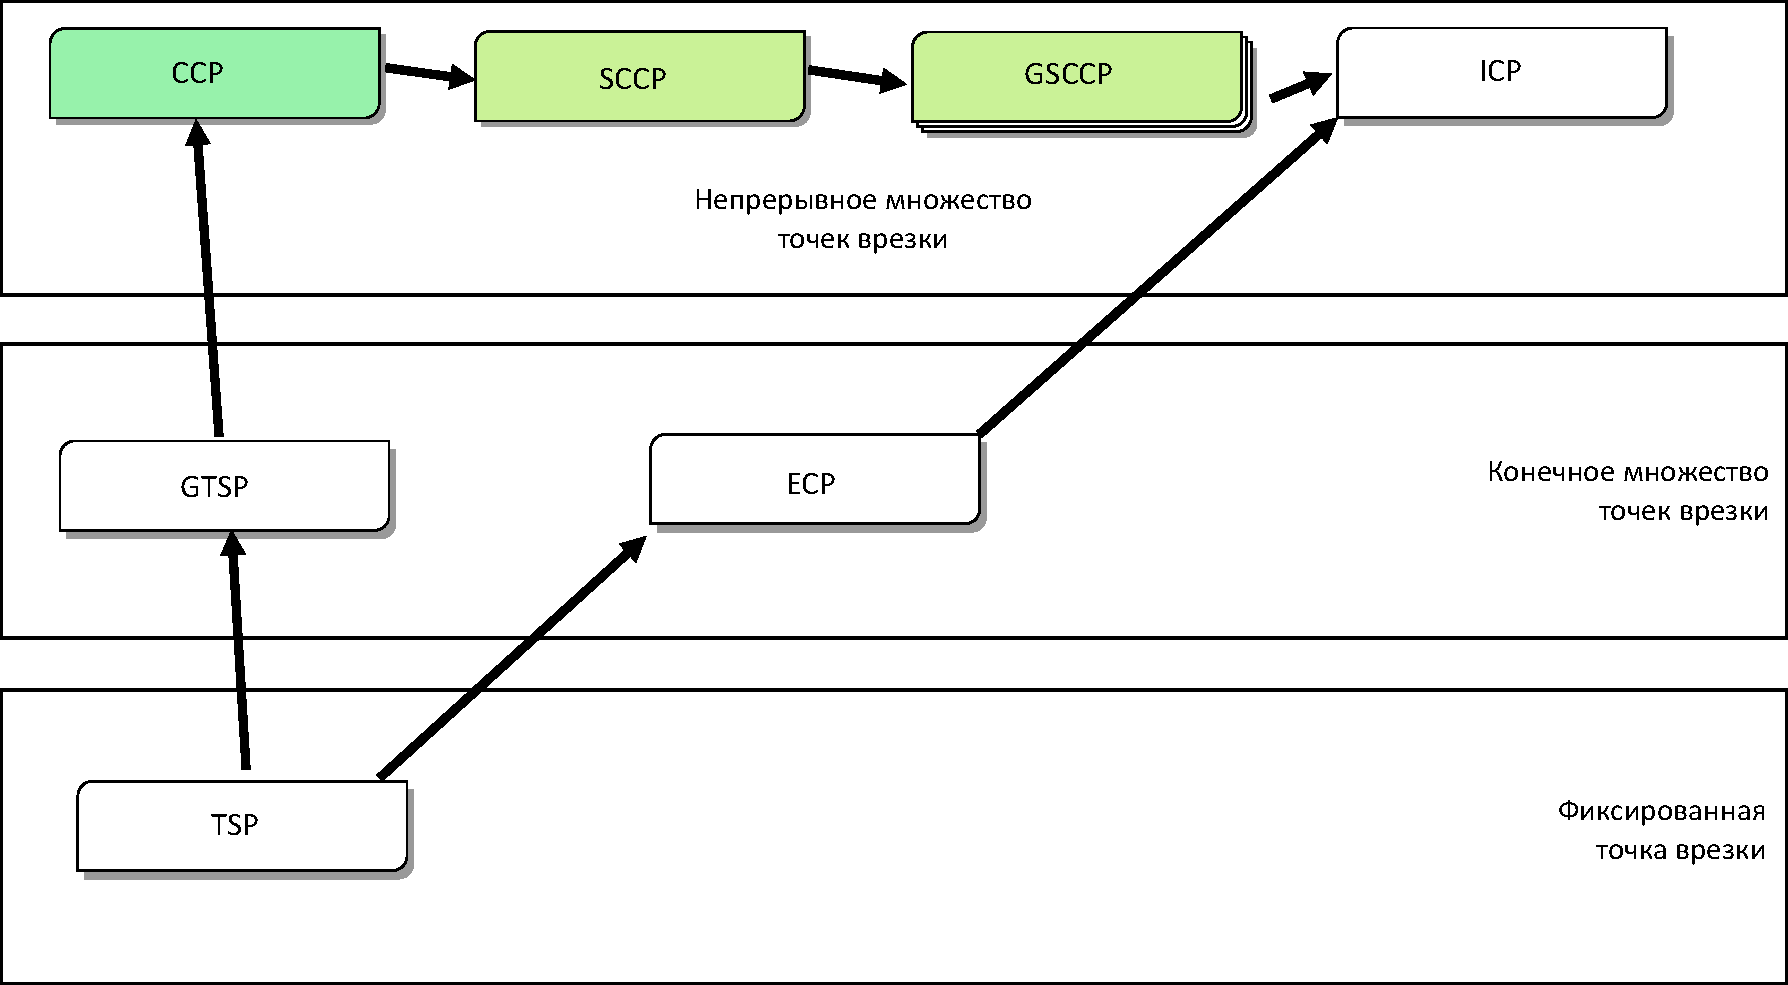
\includegraphics[width=0.95\textwidth]{classes.pdf}
  \caption{Классификация задач резки}
  \label{fig:cut-classes}
\end{figure}
